\documentclass[
ngerman,
twoside,
pdfa=false,
ruledheaders=section,%Ebene bis zu der die Überschriften mit Linien abgetrennt werden, vgl. DEMO-TUDaPub
class=report,% Basisdokumentenklasse. Wählt die Korrespondierende KOMA-Script Klasse
thesis={type=sta},% Dokumententyp Thesis, für Dissertationen siehe die Demo-Datei DEMO-TUDaPhd
accentcolor=TUDa-2c,% Auswahl der Akzentfarbe
custommargins=false,% Ränder werden mithilfe von typearea automatisch berechnet
marginpar=false,% Kopfzeile und Fußzeile erstrecken sich nicht über die Randnotizspalte
%BCOR=5mm,%Bindekorrektur, falls notwendig
parskip=half-,%Absatzkennzeichnung durch Abstand vgl. KOMA-Sript
fontsize=11pt,%Basisschriftgröße laut Corporate Design ist mit 9pt häufig zu klein
%	logofile=tuda_logo.pdf, %Falls die Logo Dateien nicht installiert sind
]{tudapub}

%%%%%%%%%%%%%%%%%%%%%%%%%%%%
% Download des TU-Logos
%%%%%%%%%%%%%%%%%%%%%%%%%%%%
% https://download.hrz.tu-darmstadt.de/protected/CE/TUDa_LaTeX/tuda_logo.pdf
% Der Pfad zum Logo kann als "logofile" angegeben werden.

%%%%%%%%%%%%%%%%%%%
% Sprachanpassung & Verbesserte Trennregeln
%%%%%%%%%%%%%%%%%%%
\usepackage[english, main=ngerman]{babel}
\usepackage[autostyle]{csquotes}% Anführungszeichen vereinfacht
\usepackage{microtype}

%%%%%%%%%%%%%%%%%%%
% Literaturverzeichnis
%%%%%%%%%%%%%%%%%%%
\usepackage{biblatex}   % Literaturverzeichnis
\addbibresource{HausarbeitBib.bib}

%%%%%%%%%%%%%%%%%%%
% Paketvorschläge Tabellen
%%%%%%%%%%%%%%%%%%%
%\usepackage{array}     % Basispaket für Tabellenkonfiguration, wird von den folgenden automatisch geladen
\usepackage{tabularx}   % Tabellen, die sich automatisch der Breite anpassen
%\usepackage{longtable} % Mehrseitige Tabellen
%\usepackage{xltabular} % Mehrseitige Tabellen mit anpassarer Breite
\usepackage{booktabs}   % Verbesserte Möglichkeiten für Tabellenlayout über horizontale Linien

%%%%%%%%%%%%%%%%%%%
% Paketvorschläge Mathematik
%%%%%%%%%%%%%%%%%%%
\usepackage{mathtools} % erweiterte Fassung von amsmath
\usepackage{amssymb}   % erweiterter Zeichensatz
\usepackage[decimalsymbol=comma]{siunitx}   % Einheiten
\usepackage{amsmath}


%%%%%%%%%%%%%%%%%
% Eigenen Pakete Gruppe01
%%%%%%%%%%%%%%%%%%%%
%\usepackage[utf8]{inputenc}
%\usepackage[ngerman]{babel}
\usepackage{hyperref}
\usepackage{graphicx}
\usepackage{subcaption}
\usepackage{listings}
\usepackage[framed, numbered]{matlab-prettifier}
%\usepackage[style=numeric]{biblatex}
%\usepackage{amsthm}
%\usepackage[squaren]{SIunits}
\usepackage{enumitem}
\usepackage{tikz}
\usepackage{pgfplots}
\usepackage{pgfplotstable}
%\usepackage{booktabs}
\pgfplotsset{compat=1.12}
\usepackage{dsfont}

\usepackage{media9}

%%%%%%%%%%%%%%%%%%%
% verschiedene Nummerierung für Abbildungen und Formeln
%%%%%%%%%%%%%%%%%%%
\usepackage{chngcntr}
\counterwithout{equation}{chapter}


%%%%%%%%%%%%%%%%%%%
% Pseudocode
%%%%%%%%%%%%%%%%%%%
\usepackage[linesnumbered,lined,boxruled]{algorithm2e} % Package für Pseudocode

%%%%%%%%%%%%%%%%%%%
% Plotting und Grafik
%%%%%%%%%%%%%%%%%%%
\usepackage{tuda-pgfplots} % Package für Plotting with TUDa mods

%%%%%%%%%%%%%%%%%%%
% Sonstiges
%%%%%%%%%%%%%%%%%%%
\usepackage{blindtext} % Package für Blindtext

\renewcommand{\tt}[1]{\texttt{#1}} 
\newcommand{\m}[1]{\textrm{#1}} 
\renewcommand{\b}[1]{\textbf{#1}} 
\newcommand{\mb}[1]{\mathbf{#1}} 

\begin{document}
	
	\title{Ausarbeitung Übung 7}
	%\subtitle{Ein Untertitel, wenn nötig}
	\author[D. Schiller, C. Kramer, S.Arnold, T. Lingenberg]{Dominik Schiller \and Constanze Kramer \and Simon Arnold \and Tobias Lingenberg} %optionales Argument ist die Signatur,
	%\reviewer{Gutachter 1 \and Gutachterin 2} %Gutachten
	
	%Diese Felder werden untereinander auf der Titelseite platziert.
	\department{} % Das Kürzel wird automatisch ersetzt und als Studienfach gewählt, siehe Liste der Kürzel im Dokument.

	
	\date{\today}
	%\examdate{\today}
	
	%	\tuprints{urn=1234,printid=12345}
	%	\dedication{Für alle, die \TeX{} nutzen.}
	
	\maketitle
	\pagenumbering{gobble} % Seitenzahlen angezeigt, startet ab dem Inhaltsverzeichnis
	
	
	%\affidavit
	%\AffidavitSignature
	%\AffidavitSignature
	
	
	%%%%%%%%%%%%%%%%%%%
	%Abstract / Kurzzusammenfassung
	%%%%%%%%%%%%%%%%%%%
	%\include{chapters/zusammenfassung}
	
	%%%%%%%%%%%%%%%%%%%
	%Inhaltsverzeichnis 
	%%%%%%%%%%%%%%%%%%%
	\cleardoublepage
	\tableofcontents % Erstellte ein Inhaltsverzeichnis
	
	%\cleardoublepage
	\pagenumbering{arabic} % Seitenzahlen angezeigt, startet ab dem Inhaltsverzeichnis
	\setcounter{page}{1} % Setzt den Seitenzahlenzähler auf 1
	
	%%%%%%%%%%%%%%%%%%%%%%%%%%%%%%%%%%%%%%%%%%%%%%%%%%%%%%%%%%%%%%%%%%%%%%%%%%%%%%%%%%%%%%%%%%%%%%%%%%
	
	% INHALT, am Besten ausgelagert in eigene Files/Kapitel und dann mit \include{Unterordner/Filename} eingefügt, sorgt für bessere Übersichtlichkeit und Fehlersuche. Einzelne Dateien sind aktuell im Ordner Sections abgelegt. 
	%%%%%%%%%%%%%%%%%%Einleitung%%%%%%%%%%%%%%%%%
	\chapter{Einleitung}\label{sec:intro}
Diese Arbeit beschäftigt sich mit dem Übungsblatt 9 des Faches \glqq Einführung in die numerische Berechnung elektromagnetischer Felder\grqq{}.
Zunächst wird der primale Divergenz und Rotationsoperator in Octave implementiert und berechnet. Anschließend wird eine Materialmatrix berechnet. Abschließend wird das Magnetfeld von zwei stromdruchflossenen Leitern in Octave simuliert. 
	%%%%%%%%%%%%%%%%%%Haupteil%%%%%%%%%%%%%%%%%%%
	\section{Dualer Divergenzoperator} 
Um das Berechnen von Potentialen und des elektrischen Feldes zu automatisieren und numerisch diese berechnen zu können, lassen sich Gebiete $\Omega$ in duale und primäre Gitter zerteilen. Die entstehenden Gitterpunkte lassen sich \glqq kanonisch\grqq{} nummerieren. Jeder dieser Punkte bekommt drei Kanten, drei Flächen und ein Volumen zugewiesen. Dies führt zwangsweise zu Geisterelementen, auf die im Folgenden noch genauer eingegangen wird. Für jede dieser Kanten $L_n$ gilt 
\begin{equation} 
	\overset{\frown}{e}_n = \int_{L_n} -\nabla\Phi \cdot d\vec{s} = \Phi(P_i)-\Phi(P_{i+1}). 
	\label{eq:e} 
\end{equation} 
Diese Beziehung nutzt man aus, um einen primären Divergenzoperator \textbf{G} zu erzeugen, der duale Divergenzoperator $\mb{\tilde{S}}$ lässt sich dann mit $\mathbf{G} = -\mathbf{\tilde{S}}^T$ berechnen. Die Einträge der Matrix \b{G} und damit auch der Matrix $\mb{\tilde{S}}$ bestehen aus 0, 1 und -1. Die Einträge von \b{G} lassen sich mit den partiellen Ableitungsoperatoren unter der Vorschrift  
\begin{equation} 
	(\mb{P}_w)_{p,q} := \delta_{p+M_w,q} - \delta{p,q} =  
	\begin{cases} -1 & \m{für    }  q = p \\ 
	 +1 & \m{für    }  q = p + M_w \\ 
	 0 & \m{sonst}	 
	\end{cases}, \m{wobei } w = x,y,z 
	\label{eq:Ableitung} 
\end{equation} 
bestimmen. \\ \\ 
Die im Anhang aufgeführte Methode \tt{fit\_dual\_div} macht genau diesen Vorgang, jedoch nicht für \b{G}, sondern für $\mb{\tilde{S}}$. Der Methode kann ein beliebiges kartesisches Gitter übergeben werden. Das Gitter wird durch die Parameter \tt{Nx, Ny, Nz} bestimmt, wobei \tt{Nx} die Anzahl an Unterteilungen in $x$-, \tt{Ny} die Anzahl an Unterteilungen in $y$- und \tt{Nz} die Anzahl an Unterteilungen in $z$-Richtung widerspiegeln. \\ \\ 
Das elektrische Feld $\vec{E}(x,y,z)$ lässt sich durch die negativen partiellen Ableitung in $x$,$y$ und $z$-Richtung des Potentials berechnen, $ \vec{E}(x,y,z) = -\nabla\Phi$. In dem vorgestellten Fall ist $\Phi(x,y,z) = x^2\sin(2\pi z)$ gegeben, daraus folgt das Elektrische Feld \\ \\ 
\begin{equation} 
	\vec{E} = \begin{pmatrix} 
	-2x\sin(2\pi z) \\ 
	0\\ 
	-2\pi x^2\cos(2\pi z) 
	\end{pmatrix} 
	. 
\end{equation} \\ \\ 
Für $(\overset{\frown}{e}_{ana})_1$ und $(\overset{\frown}{e}_{ana})_{N_p+1}$ lassen sich mit (\ref{eq:e}) konkrete Werte berechnen. Es gilt $N_x$ $=$ $N_y$ $=$ $N_z$ $=$ $2$ auf dem Gebiet $\Omega = \{-1,1\}^3$, daraus ergibt sich $N_p = 8$. Beispielhaft werden die Kanten $L_{x(1)}$ und $L_{y(1)}$ berechnet, dazu werden die Punkte $P_1 = (-1,-1,-1)^T$, $P_2 = (1,-1,-1)^T$ und $P_3 = (-1,1,-1)^T$ benötigt. Setzt man nun die Punkte entsprechend in (\ref{eq:e}) ein, so erhält man \\ \\  
\begin{equation*} 
	(\overset{\frown}{e}_{ana})_1 = \Phi(P_1) - \Phi(P_2) = 1\cdot\sin(-2\pi) - 1\cdot(-2\pi) = 0 
\end{equation*} 
und  
\begin{equation*} 
(\overset{\frown}{e}_{ana})_9 = \Phi(P_1) - \Phi(P_3) = 1\cdot\sin(-2\pi) - 1\cdot\sin(-2\pi) = 0. 
\end{equation*} 
 
Das Skript \tt{SkriptAg7\_1} berechnet die Potentiale auf dem gesamten Gebiet $\Omega$ und speichert diese in einem Vektor $\boldsymbol{\phi}$ ab, danach wird mit der Funktion \tt{fit\_dual\_div} $\mb{\tilde{S}}$ berechnet und $\mb{\overset{\frown}{e}}$ mit $ \mb{\overset{\frown}{e}} = \mb{\tilde{S}}^T\boldsymbol{\phi}$. \\ \\ 
Für die weiteren Rechnungen gilt $N_x$ $=$ $N_y$ $=$ $N_z$ $=$ $21$ und folglich $Np = 9261$. Zum Berechnen von $\overset{\frown}{e}_1$ wird die erste Zeile von $\mb{\tilde{S}}^T$ mit dem Potentialvektor $\boldsymbol{\phi}$ multipliziert, aus (\ref{eq:Ableitung}) folgert man, dass abgesehen von den ersten beiden Einträgen alle weiteren Einträge des Zeilenvektors gleich null sind. Da ein Zeilen- mit einem Spaltenvektor multipliziert wird ist das Ergebnis ein skalarer Wert
\begin{equation} 
\begin{split} 
\overset{\frown}{e}_1 &=  
\begin{bmatrix} 
1 & -1 & 0 & 0 &  \dots & 0 
\end{bmatrix} 
\begin{bmatrix} 
\phi(P_1) \\ \phi(P_2) \\ \phi(P_3) \\ \phi(P_4) \\ \vdots \\ \phi(P_{9261}) 
\end{bmatrix} \\\\ 
&= \phi(P_1) - \phi(P_2) + 0\cdot\phi(P_3) + \dots + 0\cdot\phi(P_9261) \\ 
&= \phi(P_1) - \phi(P_2) = 0 - 0 = 0. 
\end{split} 
\end{equation}\\ \\ 
Ähnlich dazu berechnet sich der Wert $\overset{\frown}{e}_{N_x+1}$. Nun wird die 22. Zeile der Matrix $\mb{\tilde{S}}^T$ gebraucht, auch diese wird dann mit dem Potentialvektor multipliziert, es ergibt sich  
\begin{equation} 
	\begin{split} 
		\overset{\frown}{e}_{22} &=  
		\begin{bmatrix} 
			0 & \dots & 0 & 1 & -1 & 0 \dots & 0 
		\end{bmatrix} 
		\begin{bmatrix} 
			\phi(P_1) \\ \vdots \\ \phi(P_{21}) \\ \phi(P_{22}) \\ \phi(P_{23}) \\ \phi(P_{24}) \\ 	\vdots 	\\ \phi(P_{9261}) 
		\end{bmatrix} 
		\\ \\ 
		&= 0\cdot\phi(P_1) + \dots + 0\cdot\phi(P_{21}) + \phi(P_{22}) - \phi(P_{23}) + 0\cdot\phi(P_{24}) + \dots + 0\cdot\phi(P_{9261}) \\ 
		&= \phi(P_{22}) - \phi(P_{23}) = 0 - 0 = 0. 
	\end{split} 
\end{equation}\\ \\ 
Die Punkte $P_1,P_2,P_{22},P_{23}$ sind durch 
\begin{equation*} 
	P_1 = \begin{pmatrix} 
	-1 \\ -1 \\ -1  
	\end{pmatrix},
	P_2 = \begin{pmatrix} 
	-0,9 \\ -1 \\ -1  
	\end{pmatrix},
	P_{22} = \begin{pmatrix} 
	-1 \\ -0,9 \\ -1
	\end{pmatrix}, 
	P_{23} = \begin{pmatrix} 
	-0,9 \\ -0,9 \\ -1  
	\end{pmatrix}
\end{equation*} gegeben. Aus diesen Beispielrechnungen wird ersichtlich, wie die Rechnung mit dem Divergenzoperator funktioniert, jede Multiplikation führt zurück zu (\ref{eq:e}). 
Die berechneten Daten für das gesamte Gebiet lassen sich mit der Simulationssoftware ParaView graphisch darstellen. In Abbildung \ref{fig:Pot} sind die entstehenden Potentiale $\phi$ zu sehen, wie erwartet ist das Potential $\phi = 0$, wenn entweder $x = 0$ gilt, oder $\sin(2\pi z) = 0$ gilt.\\ \\
Visualisiert man das Ergebnis der Berechnung des elektrischen Feldes wie in Abbildung \ref{fig:EFeld}, würde man erwarten, dass das elektrische Feld an den Rändern des Gebietes $\Omega$ gleich stark ist. Betrachtet man die Abbildung \ref{fig:EFeld}, wird deutlich, dass dies nicht der Fall ist. Auch eine Veränderung der Stärke des Feldes in $y$-Richtung würde man nicht erwarten. Die Visualisierung an den Gitterpunkten ist problematisch, da es durch die im nächsten Abschnitt vorgestellten Geisterkanten zu Rechenfehlern kommt.
\begin{figure}[h!] 
	\centering
	\includegraphics[width=.9\textwidth]{data/Potential} 
	\caption{Das entstehende Potential mit der Funktion $\Phi(x,y,z)=x^2sin(2\pi z)$ auf dem Gebiet $\Omega = \{-1,1\}^3$} 
	\label{fig:Pot} 
\end{figure} 
\begin{figure}[h!] 
	\centering
	\includegraphics[width=.9\textwidth]{data/EFeld} 
	\caption{Das entstehende elektrische Feld zu der Funktion $\Phi(x,y,z)=x^2sin(2\pi z)$ auf dem Gebiet $\Omega = \{-1,1\}^3$} 
	\label{fig:EFeld} 
\end{figure} 
 

	
\section{Geister}

Um das Rechengebiet $\Omega$, in dessen Inneren die \textsc{Maxwells}chen Gleichungen zu lösen sind, räumlich zu diskretisieren, wird es in endlich viele Teilgebiete unterteilt. Eine der gebräuchlichsten Gitterformen ist die kartesische bei der das Rechengebiet in einzelne Quader zerlegt wird. Bei Indizierung der Kanten, Flächen und Volumen mit dem kanonischen Nummerierungsschema, gibt es zu jedem Punkt drei Kanten, drei Flächen und ein Volumen. Dabei werden auch Kanten außerhalb des Rechengebiets durchnummeriert die für die spätere Lösung nicht benötigt werden. Diese nennt man Geisterkanten und findet sie immer am positiven Ende des Bereichs. Anschaulich erkennen kann man dies in Abbildung \ref{fig:geister}, der schwarze Quader ist das Rechengebiet $\Omega$, in Blau sind die Geisterkanten eingezeichnet.

\begin{figure}[thbp]
	\centering
	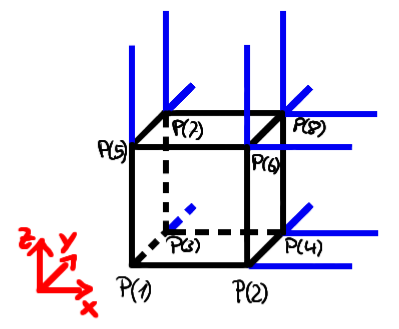
\includegraphics[width=.5\textwidth]{data/Geister}
	\caption{Einfaches Gitter mit Geisterkanten in Blau}
	\label{fig:geister}
\end{figure}

Bei einem Gitter der Größe $ N_x \times N_y \times N_z$ erhält man genau $N_x N_y + N_y N_z + N_x N_z$ Geisterkanten und -flächen, die Anzahl an Geistervolumen beträgt $N_x N_z + N_x (N_y - 1) +(N_y - 1)(N_z - 1)$. Setzt man die Geisterkanten bzw -flächen ins Verhältnis zu allen Kanten bzw Flächen so skalieren sie zu 

\begin{equation*}
	\frac{\mathrm{Geisterkanten}}{\mathrm{Alle \: Kanten}} = \frac{1}{3}(\frac{1}{N_x} + \frac{1}{N_y} + \frac{1}{N_z})
\end{equation*}

und alle Geistervolumen im Vergleich zu allen Volumen 

\begin{equation*}
		\frac{\mathrm{Geistervolumen}}{\mathrm{Alle \: Volumen}} = \frac{N_x N_y + N_y N_z + N_x N_z - N_x - N_y - N_z + 1}{N_x N_y N_z}.
\end{equation*}

Da die Geisterkanten außerhalb des Rechengebiets liegen ist es nicht nötig für diese auch das Integral zu berechnen. Für die Skizze in Abbildung \ref{fig:geister} ist es also sinnvoll nur für die schwarzen Kanten und nicht die blauen das Integral zu berechnen. Wendet man die weiter oben erwähnte Matlab-Implementierung des Gradientenoperators auf das Beispiel an so erhält man in der ersten Zeile die Potential-Differenz zwischen den Punkten $P(1)$ und $P(2)$. Zeile 2 hingegen ergibt die Potential-Differenz zwischen den Punkten $P(2)$ und $P(3)$. Diese Berechnung ist nicht sinnvoll und kommt daher, dass die eigentlich von $P(2)$ ausgehende Kante in $x$-Richtung eine Geisterkante ist. Also sollten Zeile 2 und auch alle anderen die eine Potential-Differenz diagonal durch den Quader berechnen auf null gesetzt werden.



	\section{Potentialformulierung und Eichung}
Die vier Maxwell'schen Gleichungen lauten:
\begin{equation}
\label{gl:max1}
\nabla \times \vec{E} = -\partial_t\vec{B}
\end{equation}
\begin{equation}
\label{gl:max2}
\nabla \times \left(\frac{1}{\mu_0}\vec{B}\right) = \partial_t\varepsilon_0\vec{E} + \vec{J}
\end{equation}
\begin{equation}
\label{gl:max3}
\nabla \cdot \vec{B} = 0
\end{equation}
\begin{equation}
\label{gl:max4}
\nabla \cdot \vec{E} = \frac{\rho}{\varepsilon_0}
\end{equation}
Alle Feldgrößen sind von Ort $\vec{r}$ und Zeit $t$ abhängig. Alternativ lässt sich eine Formulierung mithilfe der Potenziale $\vec{A}$ und $\Phi$ aufschreiben, welche implizit durch die Gleichungen
\begin{equation}
\label{gl:max5}
\vec{E} = -\partial_t\vec{A} - \nabla\Phi,
\end{equation}
\begin{equation}
\label{gl:max6}
\vec{B} = \nabla\times\vec{A}
\end{equation}
gegeben sind.

In der Elektrostatik kann (\ref{gl:max5}) durch $\vec{E} = - \nabla\Phi$ vereinfacht werden, da alle Vorgänge statisch sind, also zeitlich unveränderlich. Es gilt $\partial_t\vec{A} = \vec{0}$. Demnach spielen für die Elektrostatik nur Eichfelder $\vec{A}$, $\Phi$ eine Rolle, die zeitunabhängig sind.

Wir betrachten im folgenden nun jedoch den allgemeinen, zeitlich veränderlichen Fall und gehen nun näher auf die Beschreibung der Maxwell'schen Gleichungen durch die Eichfelder $\vec{A}$ und $\Phi$ ein.

(\ref{gl:max6}) impliziert (\ref{gl:max3}), da man durch Skalarmultiplikation mit dem Nabla-Operator $\nabla$

\begin{align*}
\nabla \cdot \vec{B} &= \nabla \cdot (\nabla\times\vec{A}) \\
\nabla \cdot \vec{B} &= 0
\end{align*}

erhält. Die Schreibweise $\nabla \cdot (\nabla\times\vec{A})$ ist hierbei äquivalent zur Schreibweise $\operatorname{div} \operatorname{rot} \vec{A}$, und demnach immer Null.

Ebenso impliziert (\ref{gl:max5}) die Gleichung (\ref{gl:max1}). Hierzu bildet man das Vektorprodukt mit dem Nabla-Operator $\nabla$ auf beiden Seiten der Gleichung:

\begin{align*}
\nabla \times \vec{E} &= \nabla \times (-\partial_t\vec{A} - \nabla\Phi) \\
 &= \nabla \times (-\partial_t\vec{A}) - \nabla \times(\nabla\Phi) \\
 &= \nabla \times (-\partial_t\vec{A}) \\
 &= -\partial_t (\nabla \times \vec{A}) \\
 &= -\partial_t \vec{B} \\
\end{align*}

Angewendet wurde die Rechenregel $\nabla \times(\nabla\Phi) = \operatorname{rot}\operatorname{grad}\Phi = \vec{0} $, ebenso wurde die (\ref{gl:max6}) im letzten Schritt eingesetzt, um wieder auf $\vec{B}$ zu kommen.


	%%%%%%%%%%%%%%%%%%Fazit%%%%%%%%%%%%%%%%%%%%%%
	\chapter{Fazit}\label{sec:fazit}
%\addcontentsline{toc}{section}{Fazit}
Die erste Aufgabe ergab, dass sich die beiden Leiter des Koaxialkabels wie die Platten eines Plattenkondensators verhalten. Darüber hinaus ergibt sich, dass man durch Anfügen von weiteren Segmenten an die Schaltung eine Verkleinerung der Schwingfrequenz bewirkt.
Differentialgleichungen können häufig, wie sich in Aufgabe zwei zeigt, leichter im Frequenzbereich als im Zeitbereich gelöst werden. Die durch Lösen der Differentialgleichung analytisch berechneten Ergebnisse für Zeit- und Frequenzverhalten stimmen dabei mit der numerischen Simulation durch LTSpice überein.
Die Ergebnisse der dritten Aufgabe ergeben, dass sich die Feldlinien eines Kondensators in einem Simulationskäfig nicht nur senkrecht zu den Platten bewegen, sondern dass sich auch Randeffekte an den Enden der Kondensatorplatten ausbilden. Untersucht man unterschiedliche Randbedingungen zeigt sich, dass diese sowohl den Kapazitätswert des Kondensators, als auch die elektrischen Feldlinien beeinträchtigen. Die Wahl der Simulationsrandbedingungen kann also nicht willkürlich erfolgen.
	%%%%%%%%%%%%%%%%%%Anhang%%%%%%%%%%%%%%%%%%%%%
	\chapter{Anhang}\label{sec:anhang}
\lstset{ % Octave Settings
	language=Octave,
	extendedchars=true,
	basicstyle=\footnotesize,
	numbers=left,
	numberstyle=\tiny\color{gray},
	stepnumber=1,
	numbersep=10pt,
	showspaces=false,
	showstringspaces=false,
	tabsize=2,
	breaklines=true,
	frame=single,
	morecomment = [l][\itshape\color{blue}]{\%},
	captionpos=b,
	title=\lstname
}


\lstinputlisting{data/SIS.m}
\lstinputlisting{data/SkriptAg8_2.m}
\lstinputlisting{data/SkriptAg8_3d.m}



	%%%%%%%%%%%%%%%%%%%%%%%%%%%%%%%%%%%%%%%%%%%%%%%%%%%%%%%%%%%%%%%%%%%%%%%%%%%%%%%%%%%%%%%%%%%%%%%%%%
	
	%%%%%%%%%%%%%%%%%%%
	%Abbildungs- und Tabellenverzeichnis
	%%%%%%%%%%%%%%%%%%%
	\listoffigures % Abbildungsverzeichnis (captions in den Figuren werden als Referenz genommen)
	%\listoftables % Verzeichnis der Tabellen (captions in den Tabellen werden als Referenz genommen)
	
	%%%%%%%%%%%%%%%%%%%
	%Literaturverzeichnis an dieser Stelle
	%%%%%%%%%%%%%%%%%%%
	
	
\end{document}
